\chapter{运行验证}\label{chap:demo}

\section{pageDemo 的验证思路}

为了验证页表改造是否真的生效，我写了一个 \texttt{pageDemo} 程序。它先打印一个进程内部几个典型地址：函数地址、全局变量地址、栈变量地址、几次 \texttt{malloc()} 得到的堆地址，以及 \texttt{sbrk(0)} 返回的堆尾地址。这样可以直观看到代码段、数据段、堆和栈分别落在哪些虚拟页中。

之后程序执行 \texttt{fork()}。子进程会打印 \texttt{g\_data} 和 \texttt{heap\_b} 的地址和值，然后把它们改掉；父进程等待子进程退出后，再打印同样的地址和值。如果父子进程看到的虚拟地址相同，而父进程的值没有被子进程写坏，就说明页表隔离是成立的。

\begin{lstlisting}[language=C,caption={pageDemo 中的 fork 验证逻辑},label={lst:pagedemo}]
static int g_data = 0x12345678;

pid = fork();
if (pid == 0) {
    printf("[child %d] before write\n", getpid());
    print_block("g_data", (unsigned long)&g_data);
    print_block("heap_b", (unsigned long)heap_b);
    printf("[child %d] values before: g_data=%x heap_b=%x\n",
           getpid(), g_data, *heap_b);

    g_data = 0xcafebabe;
    *heap_b = 0x0badc0de;

    printf("[child %d] values after : g_data=%x heap_b=%x\n",
           getpid(), g_data, *heap_b);
    exit(0);
}

wait(&status);

printf("[parent %d] after child exit\n", getpid());
print_block("g_data", (unsigned long)&g_data);
print_block("heap_b", (unsigned long)heap_b);
printf("[parent %d] values now   : g_data=%x heap_b=%x\n",
       getpid(), g_data, *heap_b);
\end{lstlisting}

\section{地址布局输出}

\begin{figure}[H]
  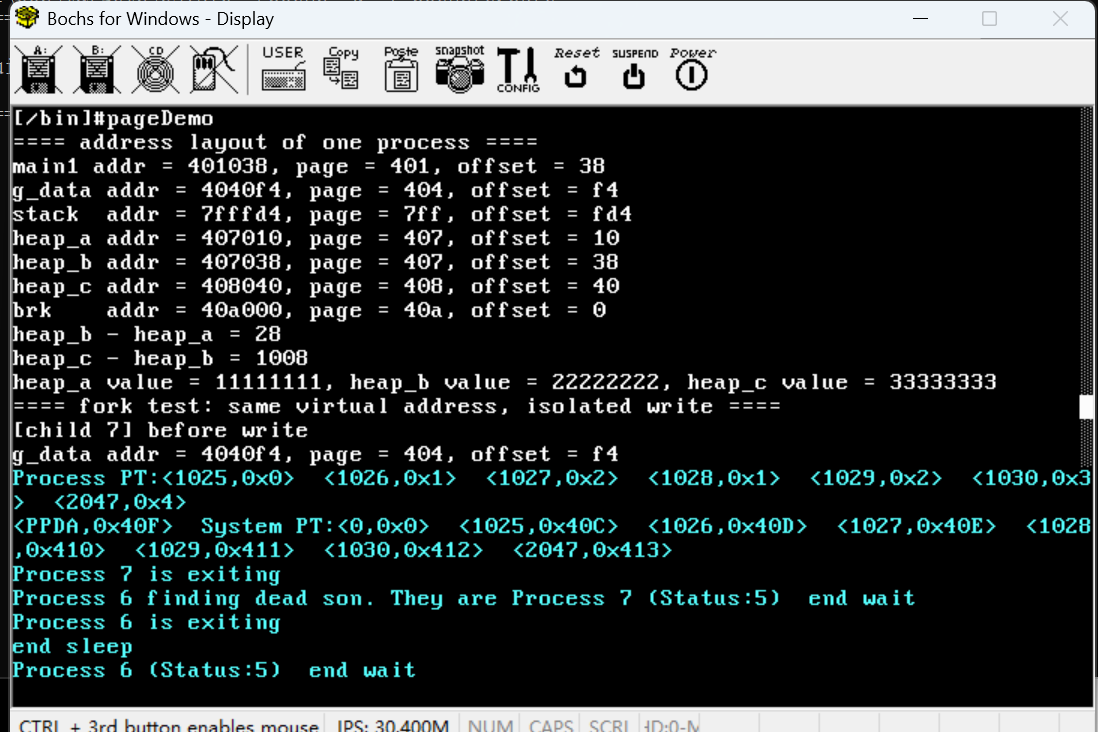
\includegraphics[width=0.95\linewidth]{figures/page_report/word_image_09.png}
  \caption{\texttt{pageDemo} 打印的进程地址布局和部分页表调试信息}
  \label{fig:pagedemo-layout}
\end{figure}

从 \figref{fig:pagedemo-layout} 可以看到，\texttt{main1} 位于页 \texttt{0x401}，全局变量 \texttt{g\_data} 位于页 \texttt{0x404}，栈变量在高地址附近的 \texttt{0x7ff} 页，堆从 \texttt{0x407}、\texttt{0x408} 继续增长，当前堆尾到了 \texttt{0x40a000}。这说明用户地址空间已经能按页观察：代码、数据、堆、栈分别落在不同逻辑页上，堆也能逐页扩张。

图中还打印了 \texttt{Process PT} 和 \texttt{System PT}。这些信息说明当前进程的用户页表内容确实参与了地址转换，而不是简单依赖一整块连续物理内存。

\section{fork 后的隔离结果}

\begin{figure}[H]
  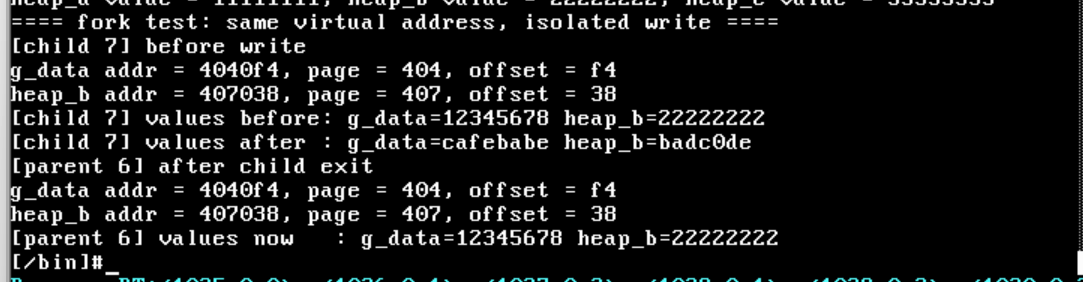
\includegraphics[width=0.95\linewidth]{figures/page_report/word_image_10.png}
  \caption{\texttt{fork()} 后父子进程同虚拟地址、写入隔离的结果}
  \label{fig:pagedemo-fork}
\end{figure}

\figref{fig:pagedemo-fork} 是最关键的结果。子进程和父进程看到的 \texttt{g\_data} 地址都是 \texttt{0x4040f4}，\texttt{heap\_b} 地址都是 \texttt{0x407038}，说明父子进程保持了同构的用户虚拟地址布局。

但子进程把 \texttt{g\_data} 改成 \texttt{cafebabe}、把 \texttt{heap\_b} 改成 \texttt{badc0de} 后，父进程再次读取时仍然得到原值 \texttt{12345678} 和 \texttt{22222222}。这就证明了当前页表设计的核心效果：虚拟地址可以相同，但底层物理页框映射已经被隔离，子进程的写入不会污染父进程。
